\section{Metodología.}\label{sec:3_metodologia}




% \subsection{Dispositivo experimental}

% En este apartado describiremos el dispositivo experimental necesario para la encapsular células individuales. Tambien, en aqeullos componentes que se 

\subsection{Chips de encapsulado.}\label{sec:chips}

Los chips que se han elegido para nuestro proyecto están fabricados en PDMS y el lugar en el  la intersección en la que se forman las gotas tienen una de geometría flujo de enfoque de tipo cuasi-planar. %El diseño de estos chips se basa en los publicados por XXX et al (REF), y un esquema de su estructura y dimensiones se muestra en la Figura~\ref{fig:chips}. 
Un esquema de su estructura y dimensiones se muestra en la Figura~\ref{fig:chips}. 
Todos los chips utilizados en este trabajo fueron fabricados en PDMS a partir de una oblea de silicio monocristalino que actúa como molde negativo. Esta oblea de silicio fue obtenida de la empresa Micrux Technologies, que la fabrico exprofeso en base a nuestro diseño en CAD por medio de fotolitografía. El procedimiento de fabricación en PDMS a partir de estas obleas se describe en el párrafo siguiente. Los diseños indicados en la Figura~\ref{fig:chips}. El diseño de la izquierda (\ref{subfig:chip3}) corresponde al chip de co-encapsulación con agarosa, utilizado para capturar las células en esferas de gel. El diseño de la derecha (\ref{subfig:chip5}) corresponde al chip de encapsulación de las esferas junto a los componentes necesarios para la elaboración de librerías genómicas. En este trabajo nos hemos centrado en la optimización del primer paso, por lo que, salvo donde se indique lo contrario, hemos utilizado chips derivados del diseño \ref{subfig:chip3}. 
Los chips que se han elegido para nuestro proyecto están fabricados en PDMS y el lugar en el que se forman las gotas tienen una de geometría flujo de enfoque de tipo planar cuasi-2D. Los chips se pueden comprar ya hechos o también, como ha sido nuestro caso, si se dispone de los medios necesarios se pueden fabricar en el laboratorio partiendo de una oblea de silicio monocristalino. En el caso de la oblea que nosotros hemos utilizado para la fabricación tiene los dos modelos de chip que se muestran en la Figura~\ref{fig:chips}.

\begin{figure}[H]
\captionsetup[subfigure]{labelformat=empty}
%Ausencia de espacios entre los subfloat, figuras en paralelo
  \begin{center} 
  
    \subfloat[]{
     \label{subfig:chip3}
     \ref{subfig:chip3}
      \includesvg[height=7.5cm]{3_metodologia/chip_3}}
    \hspace{1cm}
    \subfloat[]{
     \label{subfig:chip5}
     \ref{subfig:chip5}
      \includesvg[height=7.5cm]{3_metodologia/chip_5}}
  \end{center}
  \vspace{-5mm}
  \caption{\small Diseño de los chips grabados en la oblea de silicio que utilizada como molde para la fabricación de los chips de PDMS. Las dimensiones, en micras, están indicadas por el grosor de las líneas de control en la esquina inferior derecha de cada panel.  El diseño~\ref{subfig:chip3}  corresponde al sistema de co-encapsulación de células y agarosa. El diseño~\ref{subfig:chip5} corresponde al chip para la encapsulación simultanea de las esferas de agarosa y los reactivos para la generación de librerías genómicas. En la esta figura se pueden apreciar los distintos elementos que de los que consta cada chip. Los elementos con forma aproximadamente circulares y oscuros que se encuentran junto a pequeños puntos separados del resto de elementos del chip, son las zonas en las que se realizan los orificios para insertar los tubos. Junto a estos, también se pueden apreciar los filtros que evitan que, en algunos casos, se introduzcan elementos que atascan la zona en la que se produce el encapsulado. Los canales con forma de serpentín se comportan como amortiguadores frente a los cambios de presión y evitando que estas se transmitan de forma directa a las intersecciones entre los canales donde se juntan los fluidos. Para el chip de la Figura~\ref{subfig:chip3}, tal y como está orientado el dibujo, la entrada del aceite de encapsulado (fase continua) se sitúa en la parte superior, el orificio localizado en el centro se usa para introducir la agarosa (fase dispersa) y el situado en la parte inferior es el que se conecta el tubo de recogida. En el caso del chip de la Figura~\ref{subfig:chip5}, tenemos tres orificios de entrada para distintos fluidos o elementos que formarán la fase dispersa y un orificio situado en el extremo inferior para introducir la fase continua. El orificio de recogida, se encuentra, en este caso entre los orificios de entrada envuelto por el canal por el que circula la fase continua. Las gotas se forman en ambos chips, en unión en T que genera una intersección entre  la fase continua y la dispersa. La escala que aparece junto a cada chip está expresada en \micrometro.}
  \label{fig:chips}
\end{figure}

\subsubsection{Proceso de fabricación de los chips.}

El proceso de microfabricación que se ha llevado a cabo en este trabajo comienza partiendo de un diseño de chip impreso sobre una oblea de silicio monocristalino, el \anglicismo{wafer}. En nuestro caso los \anglicismo{wafers} se obtuvieron comercialmente a partir de la empresa Micrux Technologies, que los generó por fotolitografía de UV a partir de una máscara basada en el diseño que necesitábamos. Una vez obtenido el \anglicismo{wafer}, se utiliza como molde para genera los chips de PDMS. El PDMS se vierte sobre el \anglicismo{wafer} y una vez se ha solidificado el relieve de las estructuras impresas se transfiere como puede verse en la Figura~\ref{fig:procedimiento_pdms}.

\begin{figure}[H]
    \begin{center}
         \includegraphics[width=0.8\textwidth]{3_metodologia/pdms.png}
    \end{center}
    \caption{\small Esquema simplificado del proceso de fabricación de los chips de PDMS a partir de una oblea de silicio monocristalino. (Fuente: \url{http://www.elveflow.com/wp-content/uploads/2013/05/Soft-lithography-process-scheme.png})}
    \label{fig:procedimiento_pdms}
\end{figure}


El proceso de fabricación requiere un entorno limpio ya que incluso las pequeñas fibras de las que está hecha la ropa puede estropear las microestructuras que forman el chip. Con el objetivo de mantener el entorno lo mas limpio posible durante el proceso de microfabricación, se ha utilizado un traje de aislamiento con capucha, guantes y una careta protectora. Además, siempre que ha sido posible, se ha trabajado en una campana de flujo laminar con un filtro micométrico.

De forma esquemática y resumida los pasos que se han seguido para la fabricación de los chips son los siguientes:

\begin{itemize}

\item Se mezcla PDMS con curante en una proporción 10:1. En nuestro caso, debido al tamaño de nuestro \anglicismo{wafer} y el grosor que pretendíamos conseguir en nuestro chip (entorno a 5~mm) las cantidades exactas fueron 45~g de PDMS y 4.5~g de curante. Este proceso debe llevarse a cabo en unas condiciones de baja iluminación porque el curante es sensible a la luz. Es muy importante remover la mezcla con cuidado para evitar la formación de burbujas, pero siempre asegurándonos que la mezcla entre los componentes se está realizando correctamente.
 
\item Inevitablemente el PDMS tiene gases disueltos que podrían generar burbujas en el proceso de polimerización. Para eliminar el gas disuelto y las burbujas que se han podido formar durante el proceso anterior, se introduce la mezcla en una cámara de vacío. La mezcla permanece ahí 20~min a una presión de 50~mbar a temperatura ambiente.
 
\item Se vierte la mezcla sobre el \anglicismo{wafer}. Para evitar que el \anglicismo{wafer} se quede pegado a la placa de vidrio que lo contiene, se coloca sobre la placa una lámina de papel de aluminio y el \anglicismo{wafer} sobre esta dejando un borde sobresaliendo para poder sacarlo con facilidad. De nuevo, el \anglicismo{wafer} con el PDMS vuelve a la cámara de vacío y esta vez permanece durante unos 30 - 60~min una vez que se ha alcanzado una presión de unos 50~mbar.
 
\item La placa se introduce en la estufa a 65~\celsius\ durante 3~h - 4~h para que se endurezca. El PDMS se vuelve más quebradizo cuanto más tiempo pasa en la estufa, lo que no es conveniente para hacer los agujeros sobre el chip.
 
\item Tirando del papel de aluminio se desmolda el conjunto papel de aluminio - \anglicismo{wafer} - PDMS. Se retira el papel de aluminio y con ayuda de un bisturí se retira el PDMS que rodea el \anglicismo{wafer}. La oblea de silicio es muy dura pero quebradiza. 
 
\item En cada oblea se contenía grabados 12 chips 6 correspondientes al diseño~\ref{subfig:chip3} y otros 6 al diseño~\ref{subfig:chip5}. Con un bisturí se separan los chips de forma individual. Una vez separados se hacen los agujeros con un punzón calibrado, se limpian con isopropanol y se secan con aire a presión cerciorándonos de que quedan completamente limpios.
 
\item Se procede al pegado de los chips con los portaobjetos. Los chips de PDMS solo tienen un pequeño surco grabado por una de sus caras. Para poder trabajar con ellos debemos unirlos con otra superficie lisa y que el canal forme un tubo. El proceso de unión requiere la formación de grupos $\mathrm{O-H}$ sobre la superficie del chip y del portaobjetos, para que una vez entren en contacto ambas superficies estas queden unidas covalentemente.
 
Este proceso para la preparación de las superficies consta de dos pasos. En primer lugar se requiere limpiar la superficie de los cubreobjetos con acetona-isopropanol-agua destilada- isopropanol siguiendo este orden. El segundo paso consiste en introducir el chip y el portaobjetos en una cámara de plasma colocando las superficies que se van a unir completamente expuestas al plasma.
 
\item Los chips vuelven a la estufa y permanecen ahí un tiempo indefinido dejando que el PDMS termine de endurecerse, para posteriormente almacenarlos adecuadamente.
 
\end{itemize}

\subsection{Diseño y fabricación de la platina de microscopio.}

Para la observación del proceso de encapsulación en tiempo real, utilizamos un microscopio invertido para cultivos Zeiss Axiovert que tenía adaptada una cámara de alta velocidad %Las imágenes se tomaron en tiempo real utilizando una cámara XXXX de alta velocidad.  Brevemente, el chip se fija sobre la platina del microscopio, se acoplan las conexiones necesarias para la inyección de las células, la agarosa así como el aceite de encapsulación
Brevemente, el chip se fija sobre la platina del microscopio, se acoplan las conexiones necesarias para la inyección de las células, la agarosa así como el aceite de encapsulación.
%, y se aplican las presiones que se describen más adelante. 
Cada una de estas conexiones se conecta bien a un inyector programable de jeringa New Era 1002X, o bien a uno de los canales de salida de un controlador de presión Elveflow OB1. En el caso de los inyectores de jeringa, el fluido se introduce en el chip por medio del accionamiento del émbolo de una jeringuilla. El émbolo es programable, permitiendo la inyección de un flujo constante. En el caso de los controladores OB1, el sistema genera unos reguladores piezoeléctrios para generar, de manera regulable, presiones de entre -1 y 8 bares (tomando como referencia la presión atmosférica). Estas presiones se aplican a unos reservorios que contienen el fluido a inyectar, los cuales a su vez conectan con unos sensores de flujo. En el caso de los inyectores por jeringa, se programa un flujo continuo, que se genera por acción del émbolo. Estos sistemas son fáciles de programar, pero dado que las presiones no se monitorizan en ningún momento, pueden generar incrementos de presión dentro del circuito. Por el contrario, los controladores OB1 mantienen una presión constante, pero no necesariamente el flujo de lo que estemos inyectando. Son por tanto más complicados de poner a punto. Como se describe más adelante, una parte de este trabajo consistió en evaluar y poner a punto los distintos sistemas de inyección. Finalmente, la formación de gotas se monitoriza en tiempo real utilizando un objetivo de 10x aumentos. %El esquema completo del sistema se incluye en la Figura\ref{fig:platina_microscopio}.

Esta configuración  contiene multitud de elementos, desde los elementos que contienen las muestras y los sensores de flujo, hasta los tubos que los conectan. Es importante que todos los elementos se mantengan sobre un soporte firme que evite los movimientos relativos entre los componentes. Estos movimientos podrían modificar los flujos o impedir a la vez somos capaces de tomar imágenes o vídeos con la cámara del microscopio de las zonas de nuestro interés. Nuestro sistema controlador de flujos consistió en un generador de presiones programable Elveflow OB1. A estas presiones, cualquier cambio en la altura de los tubos produce perturbaciones en el flujo, haciendo necesario que todo el sistema se encuentre nivelado, en otro caso no vamos a conseguir flujos regulares, ya que las presiones cambiarán simplemente a medida que se llenan o vacían los tubos con fluidos utilizados. Para lograr un sistema estable y regular, capaz de estabilizar todas las conexiones, diseñamos una platina adaptada para el microscopio que contenía las sujeciones necesarias para cada uno de los elementos necesarios  (Figura\ref{fig:platina_microscopio}).

\begin{figure}[H]
    \begin{center}
         \includegraphics[width=0.8\textwidth]{3_metodologia/capas_ULTIMO2.png}
        %\includesvg[angle=-90,width=0.95\textwidth]{3_metodologia/tfm_02_bb.svg}
    \end{center}
    \caption{\small Diseño de la platina de microscopio adaptada para sujetar del chip y otros objetos utilizados durante nuestros experimentos. La platina consta de dos láminas de metacrilato superpuestas. En este dibujo, la que se encuentra sujeta al microscopio tiene los bordes de color azul. La otra, está representada con los bordes de color rojo y se encuentra sobre la lámina anterior. Los dibujo de color verde se corresponden a las perforaciones que atravesaban las dos láminas y que sirven para introducir dos tornillos que permiten mantenerlas unidas mientras permiten que la lámina superior deslice sobre la inferior en sentido vertical tal y como está orientado el dibujo. En la lamina inferior se encuentran los 3 orificios para los tornillos que sujetan la lámina al microscopio (que permiten un desplazamiento horizontal) y un cuadrado en el centro, donde se encuentran los objetivos del microscopio. La lámina superior alberga los orificios que sujetan 4 sensores de flujo (los 4 cuadrados rojos), los que sostienen 4 tubos eppendorf (los círculos rojos) y el rectángulo central que sostiene el portaobjetos con el chip pegado. Los bordes de color gris sirven para visualizar el espacio que ocupan los elementos que se pueden colocar sobre la platina. A partir de este diseño, se grabó con una fresadora controlada con control numérico por computadora (CNC) el contorno de las láminas y los orificios descritos.}
    \label{fig:platina_microscopio}
\end{figure}


A partir del diseño  de la Figura~\ref{fig:platina_microscopio}, se grabó con una fresadora controlada con control numérico por computadora (CNC) el contorno de las láminas y los orificios descritos. Esta platina mejoro notablemente la sujeción de todos los elementos que conforman nuestro dispositivo, en particular el portaobjetos sobre el que se encuentra el chip. Gracias a ello pudimos estabilizar los flujos y obtener limpiamente las imágenes y películas de formación de las microgotas. 

\subsection{Control de temperatura del circuito de agarosa.}

Uno de los desafíos fundamentales de nuestro diseño es la necesidad de co-encapsular las células diana junto a la agarosa. Este polímero debe encontrarse en fase líquida durante la fase de encapsulación, solidificándose después formando las esferas en las que capturar las células (Figura~\ref{fig:imagenes_1x} y \ref{fig:imagenes_10x}). Para ello utilizamos una agarosa low-melting (Sigma-Aldritch  39346-81-1), con un punto de fusión de 37~\celsius. Dado que la solidificación de la agarosa dentro del circuito producía importantes perturbaciones o incluso obstrucciones del flujo, fue necesario implementar un sistema que mantiene la agarosa a una temperatura constante. Para ello diseñamos y fabricamos un circuito eléctrico gobernado con una placa de Arduino.

El circuito eléctrico se puede dividir en tres partes que son esencialmente idénticas y permiten controlar la temperatura de la agarosa en tres zonas diferentes; en la jeringa, el tubo que sale de la jeringa y el extremo del tubo que esta conectado al chip. Cada una de estas partes es un sistema calefactor con su propio sensor de temperatura. 

El sensor de temperatura es en esencia un circuito que permite medir el valor de la resistencia eléctrica de un termistor NTC (por sus siglas en inglés: Negative Temperature Coefficient). El programa cargado en la placa de Arduino (ver Apéndice~\ref{apendice:codigo:arduino}) interpreta este valor de la resistencia como un cambio en la temperatura del termistor a partir de un ajuste a la ecuación

\begin{equation}
    \frac{1}{T}=A+B\ln{R}+C{(\ln{R})}^{3},
\end{equation}

siendo $T$ el valor de la temperatura absoluta, $R$ la resistencia del termistor y $A$, $B$, $C$ los coeficientes de Steinhart–Hart. En el caso específico de nuestro dispositivo, se trata del termistor NTC 3950\footnote{Los coeficientes de Steinhart–Hart se han calculado sustituyendo los valores de la resistencia del termistor proporcionados por el fabricante (254800$\Omega$ a 5~\celsius, 100000$\Omega$ a 25~\celsius y 43780$\Omega$ a 45~\celsius, que podemos consultar en la dirección web \url{https://www.makeralot.com/download/Reprap-Hotend-Thermistor-NTC-3950-100K.pdf}) en la pagina web \url{https://www.thinksrs.com/downloads/programs/therm\%20calc/ntccalibrator/ntccalculator.html} creada por Stanford Research Systems Inc} 100$\mathrm{k\Omega}$ con coeficientes $A = 0.5308572593\times{10}^{-3}$, $B = 2.396039800\times{10}^{-4}$ y $C = 0.4234340345\times{10}^{-7}$.

El sistema calefactor es una resistencia hecha con un hilo de cobre enrollado con una longitud y diámetros determinados para que disipar una potencia concreta en cada una de las partes del circuito de agarosa. Las resistencias eléctricas se encuentran conectadas en paralelo a una fuente de alimentación de 3~V. La corriente que pasa por la resistencia se controla mediante un relé que a su vez está gobernado mediante un pin digital de la placa Arduino.

La resistencia que mantiene el contenido de la jeringa a temperatura constante se compone de dos hilos de cobre de 80~cm de longitud y con una sección circular de $5\times10^{-2}\;\mathrm{mm}$ conectados en paralelo. Estos se encuentran enrollados sobre un cilindro de papel (que envuelven a la jeringa) y pegados a éste con cola de carpintero. Este conjunto, a su vez, se envuelve de nuevo con otro cilindro de papel que cumple la función de aislante térmico del entorno. Para medir la potencia disipada en la resistencia se conectó un amperímetro en serie con la resistencia. Se obtuvo un valor de 0.32~A a 3~V, por tanto la potencia disipada es de $\sim1\;\mathrm{W}$. La temperatura máxima a la que se probó que podía alcanzar era de unos 65~\celsius.

Para fabricar la resistencia que mantenía a temperatura constante el tubo que conecta la jeringa con el chip, se utilizó un cable de cobre de 4.6~m de longitud y 0.1~mm de diámetro enrollado sobre un tubo de 1~mm de diámetro externo. En este caso la potencia disipada al estar conectado a la fuente de tensión de 3~V fue de 2.5~W. Para evitar perdidas de calor y conseguir una temperatura lo más homogénea posible se envolvió conjunto tubo, cable y termistor NTC se en un tubo de plástico flexible que se comportaba como aislante térmico. El material del que está hecho el tubo que transporta la agarosa tiene un punto de fusión relativamente bajo y al subir el voltaje de la fuente de tensión a 4.5~V se observó que se fundía en ciertos puntos. En nuestros experimentos no pasó de los 45~\celsius.

En el extremo del tubo, justo antes de llegar al chip, se colocó un extrusor de plástico utilizado en impresoras 3D. Esto permite tener un control preciso de la temperatura de la agarosa antes de entrar al chip. Concretamente se utilizó un bloque de aluminio tipo MK\footnote{\url{https://inven.es/extrusores/561-bloque-aluminio-para-extrusor-mk-recambio-impresora-3d.html}}, una garganta M6 30~mm tipo MK8\footnote{\url{https://inven.es/impresoras-3d/537-garganta-m6-30mm-extrusor-mk8-recambio-impresora-3d.html}} y un bloque calentador de la cabeza\footnote{\url{https://inven.es/electronica-3d/646-bloque-calentador-de-cartucho-cabeza-de-acero-inoxidable-para-impresora-3d.html}} con una potencia de 40~W a 12~V (a 3~V la potencia disipada es de 2.3~W). Este sistema calefactor se utiliza para fundir el plástico en las impresoras 3D y sin problema alcanza temperaturas de más de 200~\celsius.
%Bloque Aluminio para Extrusor MK Recambio Impresora 3D 
%Bloque Calentador de Cartucho Cabeza de Acero Inoxidable Para Impresora 3D 
%Garganta M6 30mm Extrusor MK8

% Hay que añadir que la potencia electrica disipada en los dispositivos se encontraba muy proxima a la temperatura de equilibrio termico. 

%Se puede estimar la temperatura que va a alcanzar la resistencia en determinadas condiciones. A partir de la longitud y grosor del cable podemos estimar su volumen y conociendo el calor especifico del cobre (para todo el rango de temperaturas) de podemos aproximar la capacidad calorífica del cable en . Si la potencia disipada es de 3~W, y el proceso es adiabático, obtenemos en apenas 1~s la temperatura a aumentado en . Esto demuestra que si la resistencia no disipa el calor de forma eficaz la temperatura alcanzada por la superficie de cobre puede superar la temperatura de fusión MATERIAL, de hecho es lo que ocurrió cuando la potencia disipada se encontraba sobre los 4.5~W. 

Para realizar experimentos a mayor temperatura debemos hacer pequeños cambios que podrían afectar la programación de la placa, en las características de la resistencia calefactora o el material del que esta hecho el tubo por el que circula la agarosa. Por ejemplo se podría modificar la forma en la que se apagan y encienden los relés controlar la potencia disipada en la resistencia a fin de que la superficie de la resistencia no supere cierto valor de temperatura. En nuestro caso los relés se encuentran en la posición de circuito cerrado siempre que el sensor de temperatura sea superior a 19~\celsius\ e inferior a la temperatura que sedeamos alcanzar (la temperatura inferior debe ser una temperatura un poco inferior a la temperatura de la sala en la que realizamos los experimentos. Simplemente se ha escogido una temperatura inferior porque en caso de que el termistor este haciendo por error una medida demasiado baja, las resistencias calefactoras se encuentran apagadas y evitamos accidentes). Esta programación es la más simple, pero no es la mas acertada para determinados casos.
%El sensor de temperatura no esta midiendo la temperatura de la superficie del cobre y siempre habrá material entre el sensor de temperatura y la superficie de cobre que impide una medida directa de la temperatura, aunque solo sea material aislante\footnote{También se podría argumentar que la capacidad calorífica del termistor altera la temperatura del cable en el lugar en el que este en contacto térmico y por tanto la medida no será exacta.} que se envuelve el termistor NTC, por tanto . Entre otras muchas propuestas que se pueden hacer incluiría cambiar el material del que esta hecho el tubo por otro con mayor temperatura de fusión o cambiar el material del que esta hecho la resistencia calefactora. Típicamente el material que se utiliza para resistencias calefactoras es fibra de carbono, nicrom o resistencias flexibles de silicona para evitar las altas temperaturas que alcanza la superficie del cobre cuando se utiliza como resistencia calefactora.


\begin{figure}[H]
    \begin{center}
         \includegraphics[angle=-90,width=1\textwidth]{3_metodologia/tfm_02_bb.png}
        %\includesvg[angle=-90,width=0.95\textwidth]{3_metodologia/tfm_02_bb.svg}
    \end{center}
    \caption{\small Esquema eléctrico equivalente al utilizado en nuestra plataforma de microfluídica para mantener la temperatura de la agarosa constante. En el caso del circuito eléctrico real, no se han utilizado las placas de pruebas representadas en este esquema (más conocidas como Protoboard), la forma de las resistencias calefactoras no es la que aparece aquí y no se han utilizado pilas para alimentar a las resistencias, si no una fuente de alimentación de 3~V. Sin embargo esta representación es, bajo mi punto de vista, adecuada para entender el circuito y poder reproducirlo de nuevo si es necesario. La placa de Arduino, los pines de conexión y el modelo de relé están correctamente representados. Las resistencias representadas por su parte, tienen un valor muy próximo al de las resistencias reales, sin embargo, resistencias representadas son de un tipo que no sirve para disipar calor. Las resistencias que se encuentran junto a los termistores, están formadas por hilos de cobre de longitud y grosor específicos para obtener la resistencia eléctrica deseada.}
    \label{fig:esquema_electrico}
\end{figure}

Utilizando este circuito logramos mantener la agarosa en estado líquido durante el proceso de encapsulación. Esto permitió, como se muestra en la sección de resultados, obtener unos flujos y tamaños de encapsulado homogéneos. 


\subsection{Concentración de células de la muestra a encapsular.}\label{subsec:concentracion_celulas}

Una vez que conseguimos obtener un sistema eficaz y fiable de generación de las gotas, junto a un sistema de mantenimiento de la agarosa en estado líquido, nos planteamos el problema de la concentración óptima de células necesaria a la hora de realizar el encapsulado. El objetivo es obtener buenas frecuencias de encapsulación (que la mayoría de gotas lleven una célula) al mismo tiempo que se minimiza la frecuencia de colisión (el número de gotas que llevan dos o más células). Para optimizar este proceso elaboramos un programa en \texttt{Python}. Este programa se basa en dos axiomas: 

\begin{itemize}
    \item Las células a encapsular tienen un volumen despreciable. Se trata de una aproximación razonable ya que las células tienen un volumen ${10}^{−6}$ veces el volumen del encapsulado (diámetro de las células es de 1−2~\micrometro\ mientras que el diámetro de las gotas es 100 veces mayor.)
    
    \item La probabilidad de encontrar un célula es la misma en todo el volumen de la muestra a encapsular. La densidad de células es constante en toda la muestra.
    
\end{itemize}

%Dado que la distribución de células en la muestra es uniforme, se espera que siempre se produzca un cierto porcentaje de encapsulados múltiples (varias células en una misma \gota).
Para que los encapsulados producidos permitan hacer un análisis gnómico de células individuales, lo que tenemos que hacer es mantener el número de encapsulados múltiples por debajo de un determinado valor umbral. Nosotros hemos decidido que el número de encapsulados múltiples no debe superar el 5\% de los encapsulados individuales. 
%Por tanto la cuestión que se nos plantea ahora es: Conociendo el tamaño de las \gotas\ ¿que concentración de células debe tener la muestra para que el numero de encapsulados múltiples no supere el 5\% de los encapsulados únicos? Para responder a esta cuestión se ha escrito un \anglicismo{script} en \texttt{Python}.

El \anglicismo{script} genera un conjunto de números aleatorios, uniformemente distribuidos entre 0 y un valor dado $x$. Estos números simulan la distribución de células en la muestra y el valor $x$ su volumen. Estos puntos se pueden imaginar como puntos sobre un segmento. Para simular las \gotas\ lo que se hace es dividir el segmento en trozos, con una longitud que seria equivalente, en este caso, al volumen de las \gotas. Después se hace un recuento del número de puntos que quedan dentro de cada uno de estos trozos en los que se ha dividido el segmento y nos permite hacer una simulación de los encapsulados que se han producido en nuestra muestra. Como ya han indicado otros autores con anterioridad, la distribución de encapsulados debe responder a una distribución de Poisson. La función de Poisson es una distribución de probabilidad discreta y como tal, se encuentra normalizada. Para hacer una ajuste al número de sucesos, hay que utilizar un factor multiplicativo, que llamaremos en este caso $a$. De esta forma, el número de \gotas\ $N$ que se ha producido con $k$ células en su interior viene dado por la ecuación
\begin{equation}\label{eq:poisson}
    N(k)=a\frac{{e}^{-\lambda} {\lambda}^{k}}{k!}.
\end{equation}
$\lambda$ es el promedio de células por gota, de modo que dos distribuciones con el mismo $\lambda$ muestran la misma proporción entre el número de encapsulados de cada tipo.

El \anglicismo{script} necesita como valores de entrada un valor llamado \anglicismo{Random seed}, la densidad de células, el volumen de la muestra, el diámetro de la \gota, el flujo de la fase dispersa, el numero de simulaciones y la desviación estándar relativo al tamaño de la \gota. El valor de \anglicismo{Random seed}, es parámetro de entrada que admite la función que genera los números psudoaleatorios. Fijarlo en todas las simulaciones, nos permite garantizar la reproducibilidad de los resultados obtenidos. Los parámetros que tienen unidades físicas se deben introducir con las unidades correspondientes. Existe un paquete de la librería astropy que se encarga de hacer las transformaciones necesarias para (una vez asignadas las unidades de los parámetros de entrada) expresar siempre el resultado en las mismas unidades. El parámetro número de simulaciones, permite repetir el proceso de encapsulado de una muestra con las mismas características varias veces. La desviación estándar de la \gota\ nos permite tener en cuenta que las \gotas\ no tienen todas exactamente el mismo tamaño. Si hacemos una medida de un conjunto de \gotas\ y calculamos su desviación estándar\footnote{En este caso suponemos que la distribución de tamaños sigue una distribución normal, aunque no tiene porque ser así. Si la distribución de tamaños es diferente, se puede cambiar haciendo un pequeño cambio en el \anglicismo{script}}, podemos tener esto en cuenta para las simulaciones. Por último, el flujo de la fase dispersa, no es necesario para las simulaciones, pero nos calcula el tiempo que vamos a tardar en encapsular la muestra y la tasa de formación de las \gotas, lo son datos útiles, para por ejemplo ajustar la tasa de frames por segundo de la cámara de vídeo.

La salida proporcionada por el programa se puede ver en el Apéndice~\ref{apendice:salida}. Consiste básicamente en los valores del volumen de la \gota, la duración del experimento, la tasa de formación de las \gotas\ y las proporción en la que se ha producido cada uno de los encapsulados. La salida del \anglicismo{script} indica claramente que representa cada valor. Además se muestra el histograma de una de una de las simulaciones junto a un ajuste de la Ecuación~\ref{eq:poisson} al número de encapsulados de todas las simulaciones realizadas en una de las ejecuciones del \anglicismo{script}.


Para facilitar poder estimar la concentración de células a la muestra sin tener que recurrir a una simulación antes de cada experimento, se han escogido dos valores para la densidad de células y el diámetro de las \gotas, obtenidos mediante el \anglicismo{script} que cumplían los las condiciones que buscábamos y se ha realizado un ajustado a una curva de tipo $y=ax^{-3}$ (la densidad de células debe ser inversamente proporcional al volumen de la \gota). El ajuste resultante se muestra en la Figura~\ref{fig:rho_d} y tiene por ecuación
\begin{equation}\label{eq:rho}
    \rho=({1.87}\;{10}^{8})\times {D}^{-3}
\end{equation}
donde $\rho$ es la densidad de células por $\mathrm{mm^{-3}}$ y $D$ su diámetro expresado en micras.

\begin{figure}[H]
    \begin{center}
        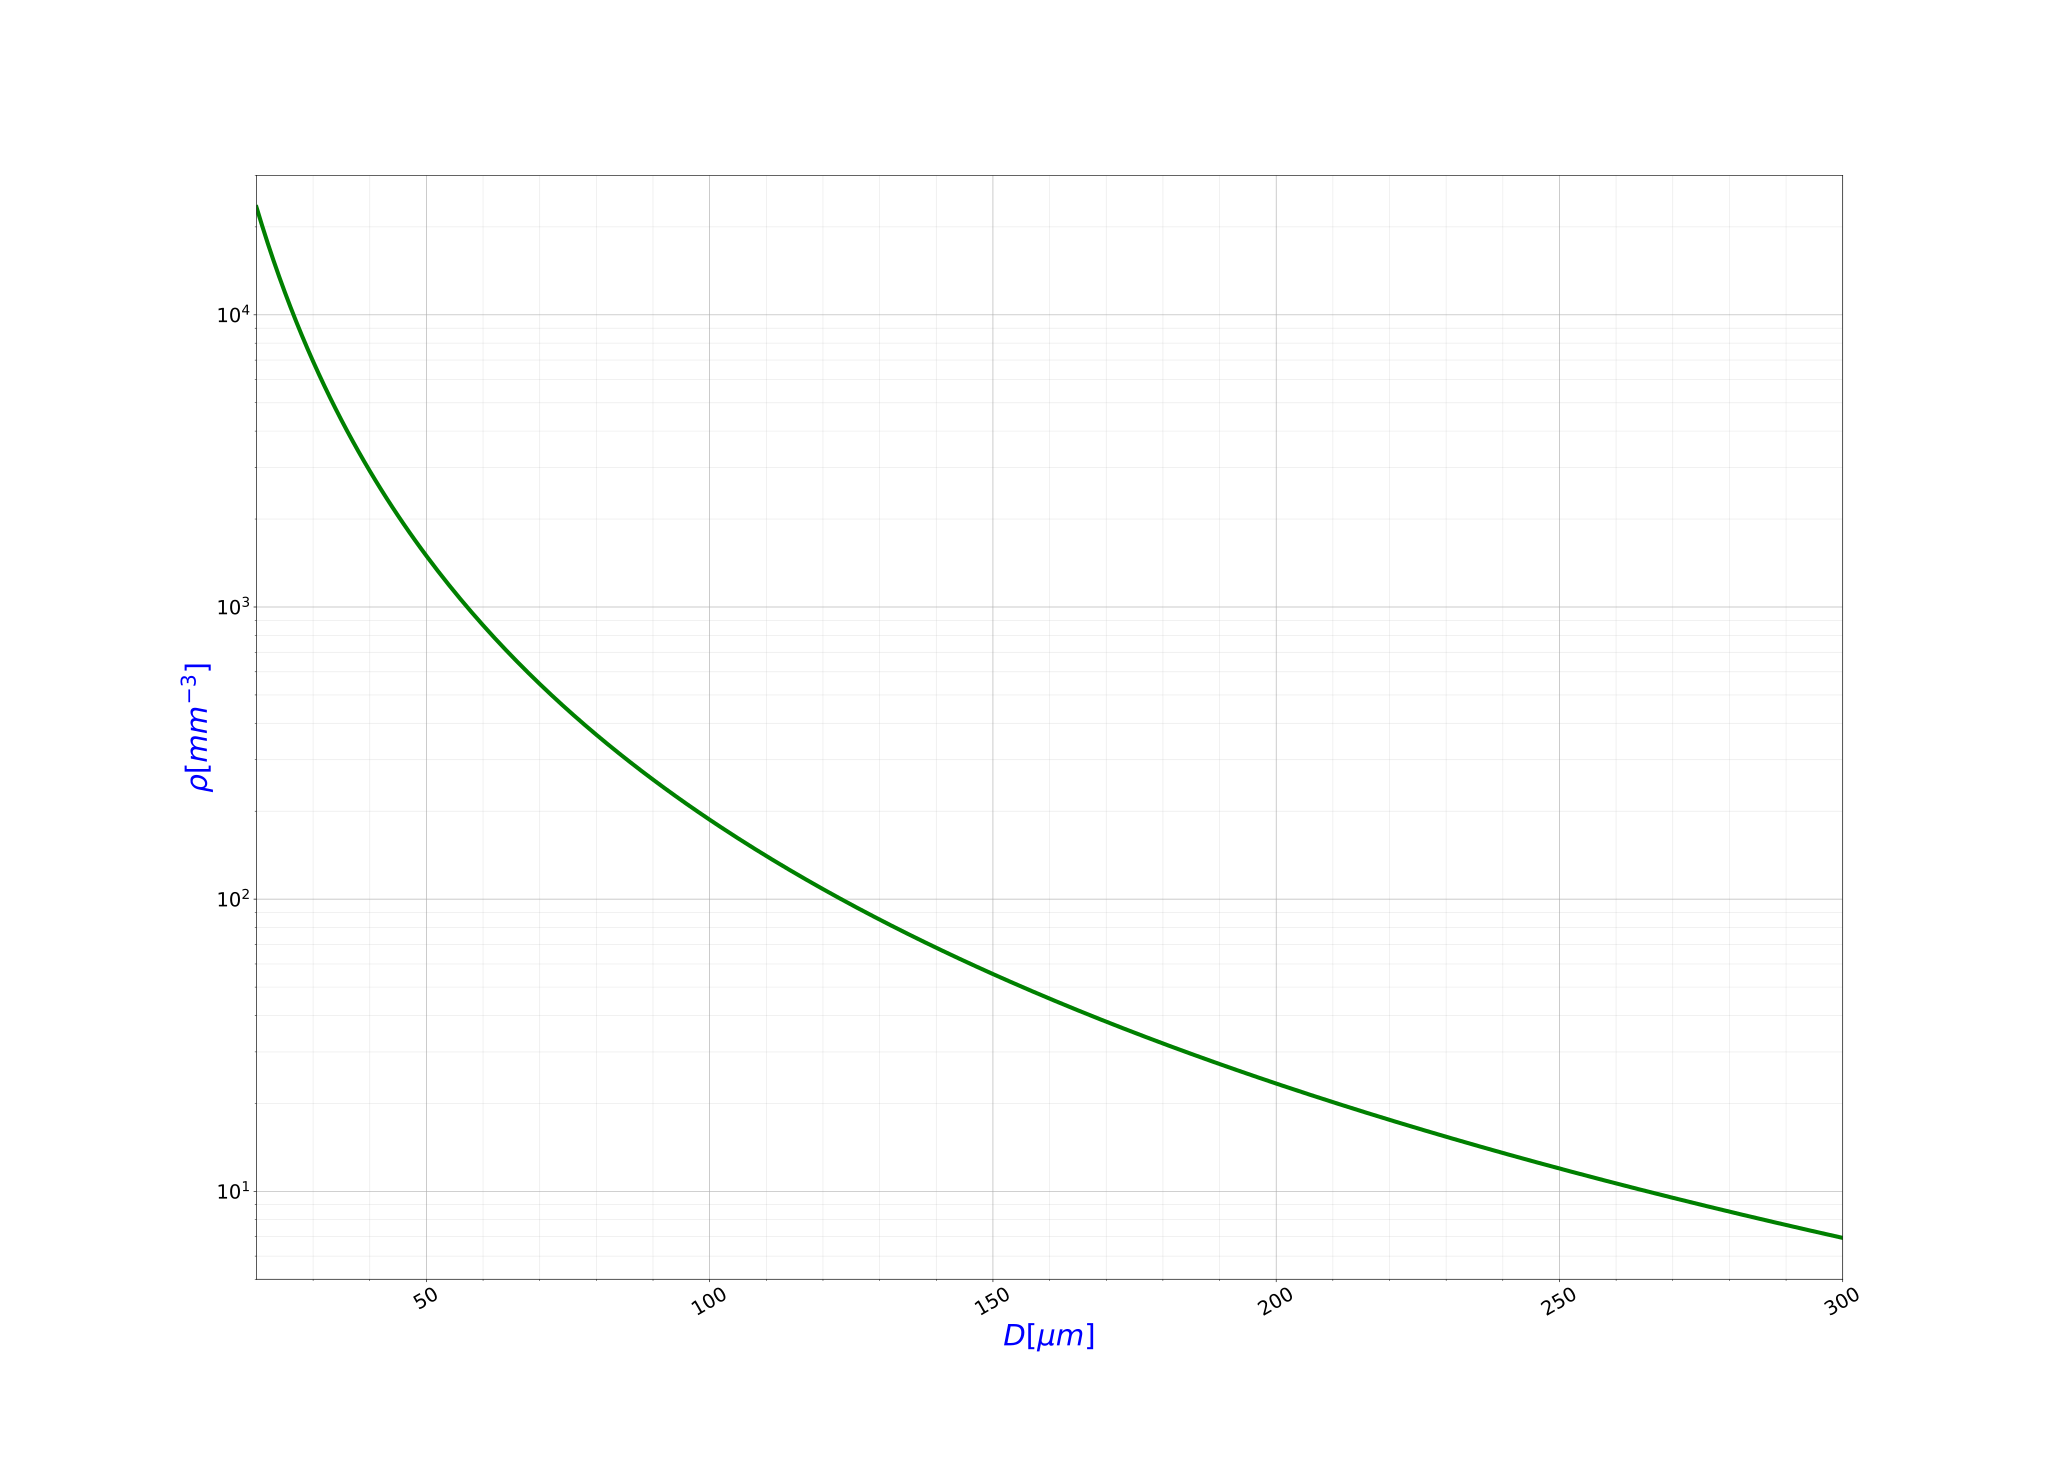
\includegraphics[width=\textwidth]{3_metodologia/curva_5_per_cent.png}
    \vspace{-15mm}
    \caption{\small Curva que relaciona el número de células $\rho$, con el diámetro de las \gotas\ $D$ a partir de un ajuste del tipo $y=ax^{-3}$ a los puntos (50,1496) (100,187). Esta curva permite el cálculo de las densidades de células en función del tamaño de las \gotas\ de modo que el número de encapsulados múltiples representa 5.15\% de los encapsulados únicos y el 4.89\% de los encapsulados totales. La distribución de encapsulados que se obtiene escogiendo $\rho$ de esta manera se ajusta es una distribución de Poisson con $\lambda=0.098$. La ecuación de la curva es la Ecuación~\ref{eq:rho}.}
    \label{fig:rho_d}
    \end{center}
\end{figure}

%Evidentemente, tamaño de las droples formadas en el sistema real no es uniforme y muestra una distribución de valores, a priori desconocida pero que se mantiene en un cierto rango. Cabe preguntarse como afecta la distribución de tamaño que adoptan las droplets a la proporción que se ha calculado entre las droplets sin encapsulado, las de encapsulado único y múltiple. En principio, podemos calcular la concentración que debería tener la muestra para aquellas que tienen un tamaño mayor y otro tamaños mas pequeños encontradas en la muestra y ver si hay alguna diferencia significativa entre las concentraciones calculadas. Si suponemos un tamaño de con valores observados máximos de y valores mínimos de vemos que estos valores son tan parecidos que están por debajo del error que comentemos a la hora de determinar la concentración de la muestra. Sin embargo resulta muy fácil hacer un programa que simule una situación en la que las droplets siguen una distribución conocida. Concretamente se ha hecho probado para el caso en el que las droplets muestran una distribución normal. En ningún sitio se ha probado en este trabajo que el tamaño responda a una distribución normal, 



\subsection{Concentración de cianobacterias en el cultivo.}

Para poder validar los resultados de nuestras simulaciones decidimos realizar encapsulaciones experimentales a distintas concentraciones celulares. Elegimos como modelo de estudio la cianobacteria unicelular Synechococcus elongatus PCC7942. Las razones para utilizar este microorganismo como modelo fueron las siguientes:

\begin{itemize}
    \item Tiene un tamaño celular de alrededor de 2 micras, lo que nos facilita el cumplimiento del axioma~1 en nuestro modelo computacional.
    \item Las cianobacterias contienen clorofila altamente fluorescente, lo que nos permitió determinar su presencia dentro de las gotas usando un microscopio de fluorescencia. Aunque las gotas son translúcidas, el coeficiente de difracción de la agarosa es muy parecido al del citoplasma celular. Esto dificulta mucho la detección de células dentro de las gotas en base a imágenes de contraste de fase. La autofluorescencia de las cianobacterias, que produce señales muy fuertes con exposiciones mínimas, nos permitió por tanto un sistema fiable de conteo. 
\end{itemize}

Las cianobacterias se crecieron en medio definido BG-11 , en condiciones de luz continua (500 mM de fotones), a 37~\celsius\ y con un 3\% de $\mathrm{CO}_{2}$ ambiental. En estas condiciones Synechococcus elongatus PCC7942 muestra un tiempo de generación de unas 4 horas. 

Para medir de manera exacta las concentraciones de células que introdujimos en cada experimento, la densidad de los cultivos se determinó mediante la cámara de Neubauer. La cámara de Neubauer es un instrumento que sirve para hacer recuentos de células en un volumen conocido, a partir de lo cual se puede determinar la densidad de células de la muestra analizada. Consta básicamente de un base de cristal sobre la que se ha grabado una rejilla de dimensiones conocidas y del tamaño similar a las células que se pretenden estudiar. Sobre esa base se coloca un cubreobjetos que al quedar apoyado sobre la base a una distancia conocida, delimita el volumen a estudiar.

Nosotros hemos utilizado para hacer los recuentos una cámara que consta de 9 cuadrados grandes de 1~mm de lado. Cada uno de estos, se encuentra a su vez subdividido en otros 16 medianos de 0.25~mm de lado. Los cuadrados medianos se vuelven a dividir, cada uno de ellos en 25 que conforman la rejilla de cuadros más pequeños, como puede verse en la Figura~\ref{fig:camara_neubauer}. 


\begin{figure}[H]
    \begin{center}
         \includegraphics[width=0.8\textwidth]{3_metodologia/plaq2.png}
         %\includesvg[angle=-90,height=15cm]{3_metodologia/curva_5_per_cent.svg}
        % \hspace{-17mm}{\includesvg[width=20cm]{3_metodologia/plaq2.png}}
    \caption{\small Representación de la base de la cámara Neubauer utilizada.(Imagen tomada de: \url{https://img.webme.com/pic/h/hematologiauis2013/plaq2.gif})}
    \label{fig:camara_neubauer}
    \end{center}
\end{figure}

La distancia a la que se encuentra el cubreobjetos de la base de la cámara es de 0.1~mm. La muestra a analizar se añade por uno de los lados de la cámara y entra por capilaridad hasta ocupar todo le volumen. Después se deja que las células se posen sobre el fondo.

Para hacer el recuento correctamente es importante utilizar la zona de la cuadrícula y el microscopio que mejor se ajusta al tamaño de las células. También es muy importante establecer un criterio para establecer qué células que se encuentran sobre alguno de los limites de la rejilla se van a contar y cuales no. Por ejemplo se puede establecer que solo se cuentan aquellas que se encuentran sobre la línea superior y lado derecho. Por último es necesario llevar un orden durante conteo para evitar dejar cuadros sin contar o contarlos dos veces. En muy fácil perderse cuando se realizan conteos mirando directamente con el microscopio, sobre todo si las células muestran pequeños desplazamientos.

Realizar recuentos mediante la cámara de Neubauer es tedioso. Para disponer de un sistema más rápido de estimación de las concentraciones de los cultivos, medimos también la densidad óptica a 750~\micrometro\ en un espectofotómetro Shimatzu UV-1580. A partir de estas medidas se elaboró una curva de calibración respecto a los resultados obtenidos en la cámara de Neubauer.

%Espectrofotómetro a 750 $\microm$

\subsection{Recuento de los encapsulados.}\label{sec:analisis_datos}

% descripción de la técnica
% microscopía confocal

Para comprobar la correlación entre las simulaciones y los resultados experimentales fue necesario desarrollar un sistema para evaluar la eficacia de los encapsulados. Para ello, como hemos apuntado antes, aprovechamos el hecho de la alta autofluorescencia de las cianobacterias dado su contenido en clorofila. De esta forma, utilizamos un microscopio de epifluorescencia Leica AXF500. Las gotas generadas por el chip se dispusieron en un portaobjetos y se analizaron con un objetivo de 10X aumentos. Tomamos imágenes en campo claro y de fluorescencia , usando para estas últimas un filtro para la fluorescencia en el canal del rojo Em 603-678 / Ex. 524-582. Dado que el tamaño de la cianobacteria es despreciable respecto al de la gota, escaneamos todo el volumen de esta realizando 30 Z-stacks. 

Los archivos obtenidos mediante esta técnica se componen de un conjunto de pares de imágenes tomadas a distintos planos; cada par tiene una imagen en el visible y otra tomada a la frecuencia emitida por la proteína fluorescente. En nuestro caso, al contener las cianobacterias clorofila, es esta la proteína que queremos encontrar para saber si el gota contiene célula en su interior o no. 

Los archivos que hemos utilizado para analizar las muestras, en nuestro caso tienen 30 planos de muestro que se toman desde la superficie de la muestra hasta poco más de los 100~\micrometro. El desplazamiento sobre el eje z (el eje vertical perpendicular a la muestra) viene determinado por el tamaño de las gotas de agarosa. El número de planos que debemos tomar lo determina el tamaño de las cianobactarias que estamos encapsulando. El tamaño típico de una cianobacteria es de 1-5~\micrometro. Lo ideal es que espaciado entre los muestreos sea inferior al tamaño del objeto que estamos buscando. Si suponemos un diametro de la gota de unos 100~\micrometro\ y tomamos 30~planos de muestreo el espaciado es de unos 3~\micrometro.

Para analizar las archivos se ha utilizado el programa Fiji Imagej. El programa cuenta con multitud de ajustes y opciones útiles que permiten poner de relieve los detalles que resultan de nuestro interés en las imágenes. Esto no supone, o no debe suponer de ningún modo la manipulación de la imagen para obtener los resultados deseados. Sin embargo es cierto que los ajustes están sujetos a cierto criterio subjetivo que dependerá de quién está realizando el análisis. Para realizar el análisis de la forma más objetiva posible, es importante establecer desde el inicio un criterio para tratar todas las imágenes de la misma forma y no modificar los archivos originales que se han realizado con el microscopio para que otro investigador pueda realizar un análisis propio, independiente del que nosotros hemos realizado.

En el caso del análisis de las imágenes a partir de las cuales se obtiene el recuento del número de encapsulados en las muestras analizadas, la manipulación que se ha realizado ha sido la proyección de la máxima intensidad alcanzada por las imágenes sobre un único plano. Las cianobacterias se han identificado como puntos rojos en la imagen de fluorescencia visibles sin necesidad de ningún otro tratamiento de la imagen. 

Para hacer el análisis se ha utilizado una herramienta de Fiji ImageJ que permite etiquetar objetos y facilita el recuento manual. Pertenecen al recuento solo las gotas de agarosa que se encontraban completamente dentro de la imagen y solo aquellas células que se encuentran dentro de esas gotas. De esta forma la muestra es algo más pequeña pero el análisis más conservador.